\section{Simulation Analysis}
\label{sec:simulation}

The following subsections present the obtained results when simulating the circuit using $Ngspice$.

\subsection{Task 1}

Table \ref{tab:sr_1} shows the simulated operating point results when t<0.

\begin{table}[h]
  \centering
  \begin{tabular}{|l|r|}
    \hline    
    {\bf Name} & {\bf Value [A or V]} \\ \hline
    v(1) & 5.169294e+00\\ \hline
v(2) & 4.893019e+00\\ \hline
v(3) & 4.311489e+00\\ \hline
v(5) & 4.932163e+00\\ \hline
v(6) & 5.799405e+00\\ \hline
v(7) & -1.89912e+00\\ \hline
v(8) & -2.87334e+00\\ \hline
@r1[i] & -2.70057e-04\\ \hline
@r2[i] & -2.82506e-04\\ \hline
@r3[i] & -1.24485e-05\\ \hline
@r4[i] & 1.206173e-03\\ \hline
@r5[i] & 2.825057e-04\\ \hline
@r6[i] & 9.361162e-04\\ \hline
@r7[i] & -9.36116e-04\\ \hline

  \end{tabular}
  \caption{Node voltages and Current in branches. Names preceeded by "@" refer to current and values are measured in A.}
  \label{tab:sr_1}
\end{table}

\subsection{Task 2}
In this subsection, an operating point analysis was made with Vs = 0 and replacing the capacitor with a voltage source, whose value derives from Vc = V6 - V8. These nodal voltages were the ones obtained in the previous task. The results can be seen in Table \ref{tab:sr_2}.

\begin{table}[h]
  \centering
  \begin{tabular}{|l|r|}
    \hline    
    {\bf Name} & {\bf Value [A or V]} \\ \hline
    v(1) & 0.000000e+00\\ \hline
v(2) & 0.000000e+00\\ \hline
v(3) & 0.000000e+00\\ \hline
v(5) & 0.000000e+00\\ \hline
v(6) & 8.672740e+00\\ \hline
v(7) & 0.000000e+00\\ \hline
v(8) & 0.000000e+00\\ \hline
@r1[i] & 0.000000e+00\\ \hline
@r2[i] & 0.000000e+00\\ \hline
@r3[i] & 0.000000e+00\\ \hline
@r4[i] & 0.000000e+00\\ \hline
@r5[i] & 2.825161e-03\\ \hline
@r6[i] & 0.000000e+00\\ \hline
@r7[i] & 0.000000e+00\\ \hline

  \end{tabular}
  \caption{Node voltages and Current in branches. Names preceeded by "@" refer to current and values are measured in A.}
  \label{tab:sr_2}
\end{table}

\subsection{Task 3}
Task 3 shows the natural response of the circuit when t=[0,20]ms. With use of previous values for $V6$ and $V8$, a transient analysis was made and the results for the natural response are shown in Figure\ref{fig:sr_3}.

\begin{figure}[h] \centering
\includegraphics[width=0.6\linewidth]{graph_1.pdf}
\caption{Natural Solution of $V6$}
\label{fig:sr_3}
\end{figure}

\subsection{Task 4}
As stated in the theorethical analysis, the total response of the circuit is the sum of natural and forced solutions. Considering $Vs$ a sinusoidal voltage source and $f = 1kHz$, we have Figure \ref{fig:sr_4} of the results for $V_{6}$ and $Vs$.

\begin{figure}[h] \centering
\includegraphics[width=0.6\linewidth]{graph_1.pdf}
\caption{Total solution of $V6$ and $Vs$}
\label{fig:sr_4}
\end{figure}

\subsection{Task 5}
In this subsection, a simulated frequency response was made. Figures \ref{fig:sr_5_1} and \ref{fig:sr_5_2} show the plotted results for the magnitude and phase of the frequency responses for $Vc$, $Vs$ and $V_{6}$.

\begin{figure}[h] \centering
\includegraphics[width=0.6\linewidth]{graph_3.pdf}
\caption{Magnitude response of $V6$, $Vs$ and $Vc$ [dB]}
\label{fig:sr_5_1}
\end{figure}

\begin{figure}[h] \centering
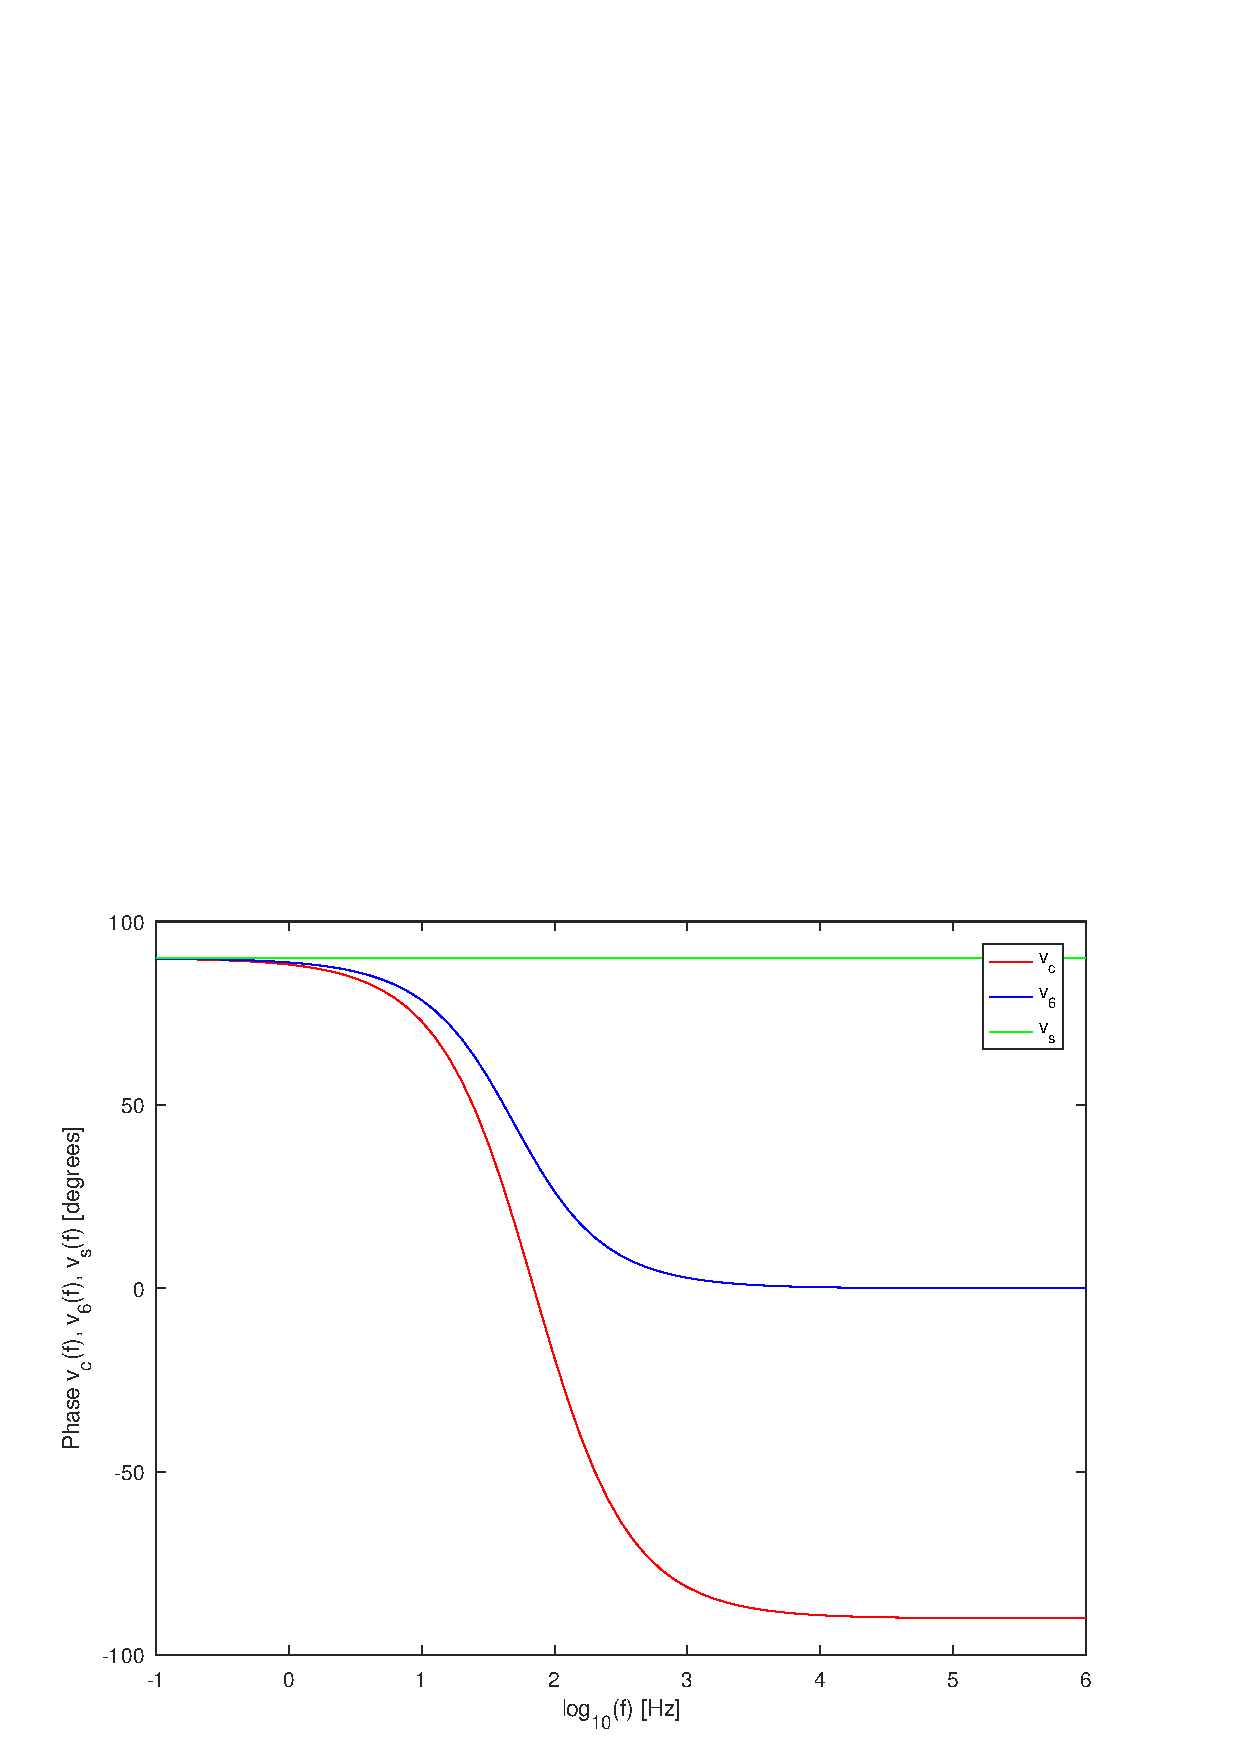
\includegraphics[width=0.6\linewidth]{phase.pdf}
\caption{Angle response of $V6$, $Vs$ and $Vc$ [degrees]}
\label{fig:sr_5_2}
\end{figure}

\subsection{Overall Results}

Comparing the theoretical and simulated results, one notices the values are very similar and in line with what was expected. Small diferences were noticed due to the approximations made in the calculations using $Octave$ tool and $Ngspice$.

Closely observing the differences between the simulated and theoretical results, the maximum relative error obtained in this assignment is a remarkably small value.

We can observe these results side by side in the following tables and graphics to better understand if the results are similar or not.

\begin{table}[h]
	\centering
	\begin{minipage}[t]{0.33\linewidth}
	 	 \begin{tabular}[t]{|l|r|}
	 	   \hline    
	 	   {\bf Name} & {\bf Value [A or V]} \\ \hline
	 	   $V1$ & 5.169294e+00 \\ \hline 
$V2$ & 4.893019e+00 \\ \hline 
$V3$ & 4.311489e+00 \\ \hline 
$V5$ & 4.932163e+00 \\ \hline 
$V6$ & 5.799405e+00 \\ \hline 
$V7$ & -1.899119e+00 \\ \hline 
$V8$ & -2.873335e+00 \\ \hline 
$I1$ & 2.700573e-04 \\ \hline 
$I2$ & 2.825057e-04 \\ \hline 
$I3$ & 1.244847e-05 \\ \hline 
$I4$ & 1.206173e-03 \\ \hline 
$I5$ & 2.825057e-04 \\ \hline 
$I6$ & 9.361162e-04 \\ \hline 
$I7$ & 9.361162e-04 \\ \hline 
$Vb$ & -3.914400e-02 \\ \hline 
$Vc$ & 0.000000e+00 \\ \hline 
$Vd$ & 6.756034e-06 \\ \hline 
$Ib$ & -2.825057e-04 \\ \hline 
$Id$ & 9.361162e-04 \\ \hline 

	 	 \end{tabular}
	 	 \label{tab:ct1}
	\end{minipage}
	\begin{minipage}[t]{0.33\linewidth}
	  		\begin{tabular}[t]{|l|r|}
	    	\hline    
	   		{\bf Name} & {\bf Value [A or V]} \\ \hline
	    	v(1) & 5.169294e+00\\ \hline
v(2) & 4.893019e+00\\ \hline
v(3) & 4.311489e+00\\ \hline
v(5) & 4.932163e+00\\ \hline
v(6) & 5.799405e+00\\ \hline
v(7) & -1.89912e+00\\ \hline
v(8) & -2.87334e+00\\ \hline
@r1[i] & -2.70057e-04\\ \hline
@r2[i] & -2.82506e-04\\ \hline
@r3[i] & -1.24485e-05\\ \hline
@r4[i] & 1.206173e-03\\ \hline
@r5[i] & 2.825057e-04\\ \hline
@r6[i] & 9.361162e-04\\ \hline
@r7[i] & -9.36116e-04\\ \hline

	  		\end{tabular}
	  	\label{tab:cs1}
	\end{minipage}
	  	\caption{Operating point for $t<0$ in Octave and NGSpice, respectivily. Names preceeded by "@" refer to current and values are measured in A.}
\end{table}

\begin{table}[h]
	\centering
	\begin{minipage}[t]{0.33\linewidth}
	 	 \begin{tabular}[t]{|l|r|}
	 	   \hline    
	 	   {\bf Name} & {\bf Value [A or V]} \\ \hline
	 	   $Vx$ & 8.672740e+00 \\ \hline 
$Ix$ & 2.825161e-03 \\ \hline 
$Req$ & 3.069821e+03 \\ \hline 
$Time Constant$ & 3.218747e-03 \\ \hline 
$V1$ & 0.000000e+00 \\ \hline 
$V2$ & 0.000000e+00 \\ \hline 
$V3$ & 0.000000e+00 \\ \hline 
$V5$ & 0.000000e+00 \\ \hline 
$V6$ & 8.672740e+00 \\ \hline 
$V7$ & 0.000000e+00 \\ \hline 
$V8$ & -0.000000e+00 \\ \hline 
$I1$ & 0.000000e+00 \\ \hline 
$I2$ & 0.000000e+00 \\ \hline 
$I3$ & 0.000000e+00 \\ \hline 
$I4$ & 0.000000e+00 \\ \hline 
$I5$ & 2.825161e-03 \\ \hline 
$I6$ & -0.000000e+00 \\ \hline 
$I7$ & 0.000000e+00 \\ \hline 
$Vb$ & -0.000000e+00 \\ \hline 
$Vd$ & 0.000000e+00 \\ \hline 
$Ib$ & -0.000000e+00 \\ \hline 
$Id$ & 0.000000e+00 \\ \hline 

	 	 \end{tabular}
	 	 \label{tab:ct2}
	\end{minipage}
	\begin{minipage}[t]{0.33\linewidth}
	  		\begin{tabular}[t]{|l|r|}
	    	\hline    
	   		{\bf Name} & {\bf Value [A or V]} \\ \hline
	    	v(1) & 0.000000e+00\\ \hline
v(2) & 0.000000e+00\\ \hline
v(3) & 0.000000e+00\\ \hline
v(5) & 0.000000e+00\\ \hline
v(6) & 8.672740e+00\\ \hline
v(7) & 0.000000e+00\\ \hline
v(8) & 0.000000e+00\\ \hline
@r1[i] & 0.000000e+00\\ \hline
@r2[i] & 0.000000e+00\\ \hline
@r3[i] & 0.000000e+00\\ \hline
@r4[i] & 0.000000e+00\\ \hline
@r5[i] & 2.825161e-03\\ \hline
@r6[i] & 0.000000e+00\\ \hline
@r7[i] & 0.000000e+00\\ \hline

	  		\end{tabular}
	  	\label{tab:cs2}
	\end{minipage}
	  	\caption{Operating point for $t=0$ in Octave and NGSpice, respectivily. Names preceeded by "@" refer to current and values are measured in A.}
\end{table}

\vspace{10cm}
